% Options for packages loaded elsewhere
% Options for packages loaded elsewhere
\PassOptionsToPackage{unicode}{hyperref}
\PassOptionsToPackage{hyphens}{url}
\PassOptionsToPackage{dvipsnames,svgnames,x11names}{xcolor}
%
\documentclass[
  letterpaper,
  DIV=11,
  numbers=noendperiod]{scrartcl}
\usepackage{xcolor}
\usepackage{amsmath,amssymb}
\setcounter{secnumdepth}{-\maxdimen} % remove section numbering
\usepackage{iftex}
\ifPDFTeX
  \usepackage[T1]{fontenc}
  \usepackage[utf8]{inputenc}
  \usepackage{textcomp} % provide euro and other symbols
\else % if luatex or xetex
  \usepackage{unicode-math} % this also loads fontspec
  \defaultfontfeatures{Scale=MatchLowercase}
  \defaultfontfeatures[\rmfamily]{Ligatures=TeX,Scale=1}
\fi
\usepackage{lmodern}
\ifPDFTeX\else
  % xetex/luatex font selection
\fi
% Use upquote if available, for straight quotes in verbatim environments
\IfFileExists{upquote.sty}{\usepackage{upquote}}{}
\IfFileExists{microtype.sty}{% use microtype if available
  \usepackage[]{microtype}
  \UseMicrotypeSet[protrusion]{basicmath} % disable protrusion for tt fonts
}{}
\makeatletter
\@ifundefined{KOMAClassName}{% if non-KOMA class
  \IfFileExists{parskip.sty}{%
    \usepackage{parskip}
  }{% else
    \setlength{\parindent}{0pt}
    \setlength{\parskip}{6pt plus 2pt minus 1pt}}
}{% if KOMA class
  \KOMAoptions{parskip=half}}
\makeatother
% Make \paragraph and \subparagraph free-standing
\makeatletter
\ifx\paragraph\undefined\else
  \let\oldparagraph\paragraph
  \renewcommand{\paragraph}{
    \@ifstar
      \xxxParagraphStar
      \xxxParagraphNoStar
  }
  \newcommand{\xxxParagraphStar}[1]{\oldparagraph*{#1}\mbox{}}
  \newcommand{\xxxParagraphNoStar}[1]{\oldparagraph{#1}\mbox{}}
\fi
\ifx\subparagraph\undefined\else
  \let\oldsubparagraph\subparagraph
  \renewcommand{\subparagraph}{
    \@ifstar
      \xxxSubParagraphStar
      \xxxSubParagraphNoStar
  }
  \newcommand{\xxxSubParagraphStar}[1]{\oldsubparagraph*{#1}\mbox{}}
  \newcommand{\xxxSubParagraphNoStar}[1]{\oldsubparagraph{#1}\mbox{}}
\fi
\makeatother

\usepackage{color}
\usepackage{fancyvrb}
\newcommand{\VerbBar}{|}
\newcommand{\VERB}{\Verb[commandchars=\\\{\}]}
\DefineVerbatimEnvironment{Highlighting}{Verbatim}{commandchars=\\\{\}}
% Add ',fontsize=\small' for more characters per line
\usepackage{framed}
\definecolor{shadecolor}{RGB}{241,243,245}
\newenvironment{Shaded}{\begin{snugshade}}{\end{snugshade}}
\newcommand{\AlertTok}[1]{\textcolor[rgb]{0.68,0.00,0.00}{#1}}
\newcommand{\AnnotationTok}[1]{\textcolor[rgb]{0.37,0.37,0.37}{#1}}
\newcommand{\AttributeTok}[1]{\textcolor[rgb]{0.40,0.45,0.13}{#1}}
\newcommand{\BaseNTok}[1]{\textcolor[rgb]{0.68,0.00,0.00}{#1}}
\newcommand{\BuiltInTok}[1]{\textcolor[rgb]{0.00,0.23,0.31}{#1}}
\newcommand{\CharTok}[1]{\textcolor[rgb]{0.13,0.47,0.30}{#1}}
\newcommand{\CommentTok}[1]{\textcolor[rgb]{0.37,0.37,0.37}{#1}}
\newcommand{\CommentVarTok}[1]{\textcolor[rgb]{0.37,0.37,0.37}{\textit{#1}}}
\newcommand{\ConstantTok}[1]{\textcolor[rgb]{0.56,0.35,0.01}{#1}}
\newcommand{\ControlFlowTok}[1]{\textcolor[rgb]{0.00,0.23,0.31}{\textbf{#1}}}
\newcommand{\DataTypeTok}[1]{\textcolor[rgb]{0.68,0.00,0.00}{#1}}
\newcommand{\DecValTok}[1]{\textcolor[rgb]{0.68,0.00,0.00}{#1}}
\newcommand{\DocumentationTok}[1]{\textcolor[rgb]{0.37,0.37,0.37}{\textit{#1}}}
\newcommand{\ErrorTok}[1]{\textcolor[rgb]{0.68,0.00,0.00}{#1}}
\newcommand{\ExtensionTok}[1]{\textcolor[rgb]{0.00,0.23,0.31}{#1}}
\newcommand{\FloatTok}[1]{\textcolor[rgb]{0.68,0.00,0.00}{#1}}
\newcommand{\FunctionTok}[1]{\textcolor[rgb]{0.28,0.35,0.67}{#1}}
\newcommand{\ImportTok}[1]{\textcolor[rgb]{0.00,0.46,0.62}{#1}}
\newcommand{\InformationTok}[1]{\textcolor[rgb]{0.37,0.37,0.37}{#1}}
\newcommand{\KeywordTok}[1]{\textcolor[rgb]{0.00,0.23,0.31}{\textbf{#1}}}
\newcommand{\NormalTok}[1]{\textcolor[rgb]{0.00,0.23,0.31}{#1}}
\newcommand{\OperatorTok}[1]{\textcolor[rgb]{0.37,0.37,0.37}{#1}}
\newcommand{\OtherTok}[1]{\textcolor[rgb]{0.00,0.23,0.31}{#1}}
\newcommand{\PreprocessorTok}[1]{\textcolor[rgb]{0.68,0.00,0.00}{#1}}
\newcommand{\RegionMarkerTok}[1]{\textcolor[rgb]{0.00,0.23,0.31}{#1}}
\newcommand{\SpecialCharTok}[1]{\textcolor[rgb]{0.37,0.37,0.37}{#1}}
\newcommand{\SpecialStringTok}[1]{\textcolor[rgb]{0.13,0.47,0.30}{#1}}
\newcommand{\StringTok}[1]{\textcolor[rgb]{0.13,0.47,0.30}{#1}}
\newcommand{\VariableTok}[1]{\textcolor[rgb]{0.07,0.07,0.07}{#1}}
\newcommand{\VerbatimStringTok}[1]{\textcolor[rgb]{0.13,0.47,0.30}{#1}}
\newcommand{\WarningTok}[1]{\textcolor[rgb]{0.37,0.37,0.37}{\textit{#1}}}

\usepackage{longtable,booktabs,array}
\usepackage{calc} % for calculating minipage widths
% Correct order of tables after \paragraph or \subparagraph
\usepackage{etoolbox}
\makeatletter
\patchcmd\longtable{\par}{\if@noskipsec\mbox{}\fi\par}{}{}
\makeatother
% Allow footnotes in longtable head/foot
\IfFileExists{footnotehyper.sty}{\usepackage{footnotehyper}}{\usepackage{footnote}}
\makesavenoteenv{longtable}
\usepackage{graphicx}
\makeatletter
\newsavebox\pandoc@box
\newcommand*\pandocbounded[1]{% scales image to fit in text height/width
  \sbox\pandoc@box{#1}%
  \Gscale@div\@tempa{\textheight}{\dimexpr\ht\pandoc@box+\dp\pandoc@box\relax}%
  \Gscale@div\@tempb{\linewidth}{\wd\pandoc@box}%
  \ifdim\@tempb\p@<\@tempa\p@\let\@tempa\@tempb\fi% select the smaller of both
  \ifdim\@tempa\p@<\p@\scalebox{\@tempa}{\usebox\pandoc@box}%
  \else\usebox{\pandoc@box}%
  \fi%
}
% Set default figure placement to htbp
\def\fps@figure{htbp}
\makeatother





\setlength{\emergencystretch}{3em} % prevent overfull lines

\providecommand{\tightlist}{%
  \setlength{\itemsep}{0pt}\setlength{\parskip}{0pt}}



 


\KOMAoption{captions}{tableheading}
\makeatletter
\@ifpackageloaded{caption}{}{\usepackage{caption}}
\AtBeginDocument{%
\ifdefined\contentsname
  \renewcommand*\contentsname{Table of contents}
\else
  \newcommand\contentsname{Table of contents}
\fi
\ifdefined\listfigurename
  \renewcommand*\listfigurename{List of Figures}
\else
  \newcommand\listfigurename{List of Figures}
\fi
\ifdefined\listtablename
  \renewcommand*\listtablename{List of Tables}
\else
  \newcommand\listtablename{List of Tables}
\fi
\ifdefined\figurename
  \renewcommand*\figurename{Figure}
\else
  \newcommand\figurename{Figure}
\fi
\ifdefined\tablename
  \renewcommand*\tablename{Table}
\else
  \newcommand\tablename{Table}
\fi
}
\@ifpackageloaded{float}{}{\usepackage{float}}
\floatstyle{ruled}
\@ifundefined{c@chapter}{\newfloat{codelisting}{h}{lop}}{\newfloat{codelisting}{h}{lop}[chapter]}
\floatname{codelisting}{Listing}
\newcommand*\listoflistings{\listof{codelisting}{List of Listings}}
\makeatother
\makeatletter
\makeatother
\makeatletter
\@ifpackageloaded{caption}{}{\usepackage{caption}}
\@ifpackageloaded{subcaption}{}{\usepackage{subcaption}}
\makeatother
\usepackage{bookmark}
\IfFileExists{xurl.sty}{\usepackage{xurl}}{} % add URL line breaks if available
\urlstyle{same}
\hypersetup{
  pdftitle={Sentiment Analysis on Obama and Trump Tweets},
  colorlinks=true,
  linkcolor={blue},
  filecolor={Maroon},
  citecolor={Blue},
  urlcolor={Blue},
  pdfcreator={LaTeX via pandoc}}


\title{Sentiment Analysis on Obama and Trump Tweets}
\author{}
\date{}
\begin{document}
\maketitle


\subsection{Introduction}\label{introduction}

We are interested in how former president Obama and Trump tweet on their
personal account. Along with their access to the @POTUS account on
Twitter, they also had access to their own personal account. Since
@POTUS is the official account for the President of the United States, I
was less curious in exploring what they tweeted on this particular
account during their presidency; instead, I was interested in what both
Obama and Trump would tweet on their personal Twitter accounts. Although
both Obama's and Trump's Twitter accounts were monitored, they had more
freedom on what they posted on their personal accounts rather than the
@POTUS account. In this project, I will explore the differences in how
Obama and Trump would tweet during their presidency. We begin by data
wrangling both
\href{https://www.kaggle.com/datasets/neelgajare/all-12000-president-obama-tweets}{Obama's}
and
\href{https://www.kaggle.com/datasets/zusmani/trumps-legacy}{Trump's}
tweets in order to make meaningful analyses. During this process, I have
decided to only include the years of their respective presidency terms.
I felt it was more important to analyse how they interacted with the
media when they were representing our country.

\begin{Shaded}
\begin{Highlighting}[]
\CommentTok{\#wrangling Trump\textquotesingle{}s tweets}
\NormalTok{trump\_tweets\_ym }\OtherTok{\textless{}{-}} \FunctionTok{read\_csv}\NormalTok{(}\StringTok{"\textasciitilde{}/Desktop/SDSProjects/maryw{-}1.github.io/Trumps\_Legcy.csv"}\NormalTok{) }\SpecialCharTok{|\textgreater{}}
  \FunctionTok{mutate}\NormalTok{(}\AttributeTok{timestamp =} \FunctionTok{mdy\_hm}\NormalTok{(date),}
         \AttributeTok{year =} \FunctionTok{str\_extract}\NormalTok{(timestamp, }\StringTok{"(}\SpecialCharTok{\textbackslash{}\textbackslash{}}\StringTok{d\{4\})"}\NormalTok{)) }\SpecialCharTok{|\textgreater{}}
  \FunctionTok{filter}\NormalTok{(year }\SpecialCharTok{\textgreater{}=} \DecValTok{2016}\NormalTok{) }\SpecialCharTok{|\textgreater{}}
  \FunctionTok{mutate}\NormalTok{(}\AttributeTok{timestamp =} \FunctionTok{as.Date}\NormalTok{(}\FunctionTok{mdy\_hm}\NormalTok{(date)),}
         \AttributeTok{year\_month =} \FunctionTok{str\_extract}\NormalTok{(timestamp, }\StringTok{"(}\SpecialCharTok{\textbackslash{}\textbackslash{}}\StringTok{d\{4\}{-}}\SpecialCharTok{\textbackslash{}\textbackslash{}}\StringTok{d\{2\})"}\NormalTok{), }
         \AttributeTok{year\_month =} \FunctionTok{ym}\NormalTok{(year\_month), }
         \AttributeTok{president =} \StringTok{\textquotesingle{}Trump\textquotesingle{}}\NormalTok{) }\SpecialCharTok{|\textgreater{}}
  \FunctionTok{rename}\NormalTok{(}\AttributeTok{tweet =}\NormalTok{ text) }\SpecialCharTok{|\textgreater{}} 
  \FunctionTok{select}\NormalTok{(timestamp, tweet, year\_month, president, year) }
  
\CommentTok{\#wrangling Obama\textquotesingle{}s tweets }
\NormalTok{obama\_tweets\_ym }\OtherTok{\textless{}{-}} \FunctionTok{read\_csv}\NormalTok{(}\StringTok{"\textasciitilde{}/Desktop/SDSProjects/maryw{-}1.github.io/obama.csv"}\NormalTok{) }\SpecialCharTok{|\textgreater{}}
    \FunctionTok{mutate}\NormalTok{(}\AttributeTok{year =} \FunctionTok{str\_extract}\NormalTok{(Timestamp, }\StringTok{"(}\SpecialCharTok{\textbackslash{}\textbackslash{}}\StringTok{d\{4\})"}\NormalTok{),}
           \AttributeTok{year =} \FunctionTok{as.numeric}\NormalTok{(year),}
           \AttributeTok{president =} \StringTok{"Obama"}\NormalTok{) }\SpecialCharTok{|\textgreater{}} 
  \FunctionTok{filter}\NormalTok{(year }\SpecialCharTok{\textgreater{}=} \DecValTok{2006}\NormalTok{ , year }\SpecialCharTok{\textless{}=} \DecValTok{2017}\NormalTok{) }\SpecialCharTok{|\textgreater{}}
  \FunctionTok{mutate}\NormalTok{(}\AttributeTok{year\_month =} \FunctionTok{str\_extract}\NormalTok{(Timestamp,}\StringTok{"(}\SpecialCharTok{\textbackslash{}\textbackslash{}}\StringTok{d\{4\}{-}}\SpecialCharTok{\textbackslash{}\textbackslash{}}\StringTok{d\{2\})"}\NormalTok{),}
         \AttributeTok{year\_month =} \FunctionTok{ym}\NormalTok{(year\_month)) }\SpecialCharTok{|\textgreater{}} 
  \FunctionTok{rename}\NormalTok{(}\AttributeTok{tweet =}\NormalTok{ Embedded\_text,}
         \AttributeTok{timestamp =}\NormalTok{ Timestamp) }\SpecialCharTok{|\textgreater{}}
  \FunctionTok{select}\NormalTok{(timestamp, tweet, year\_month, president, year) }

\CommentTok{\#combining the two datasets together; }
\NormalTok{obama\_and\_trump }\OtherTok{\textless{}{-}} \FunctionTok{rbind}\NormalTok{(obama\_tweets\_ym, trump\_tweets\_ym)}
\end{Highlighting}
\end{Shaded}

Before we do any sentiment analysis, let us analyse how many tweets
Obama and Trump tweeted during their presidency.

\begin{Shaded}
\begin{Highlighting}[]
\NormalTok{obama\_and\_trump }\SpecialCharTok{|\textgreater{}}
  \FunctionTok{group\_by}\NormalTok{(president) }\SpecialCharTok{|\textgreater{}}
  \FunctionTok{count}\NormalTok{() }\SpecialCharTok{|\textgreater{}}
  \FunctionTok{ggplot}\NormalTok{(}\FunctionTok{aes}\NormalTok{(}\AttributeTok{x =}\NormalTok{ president, }\AttributeTok{y =}\NormalTok{ n)) }\SpecialCharTok{+}
  \FunctionTok{geom\_col}\NormalTok{() }\SpecialCharTok{+}
  \FunctionTok{labs}\NormalTok{( }
       \AttributeTok{x =} \StringTok{"President"}\NormalTok{, }
       \AttributeTok{y =} \StringTok{"Number of Tweets"}\NormalTok{,}
       \AttributeTok{title =} \StringTok{"Number of Tweets by President"}\NormalTok{,}
       \AttributeTok{subtitle =} \StringTok{"During their respective presidential terms"}\NormalTok{)}
\end{Highlighting}
\end{Shaded}

\pandocbounded{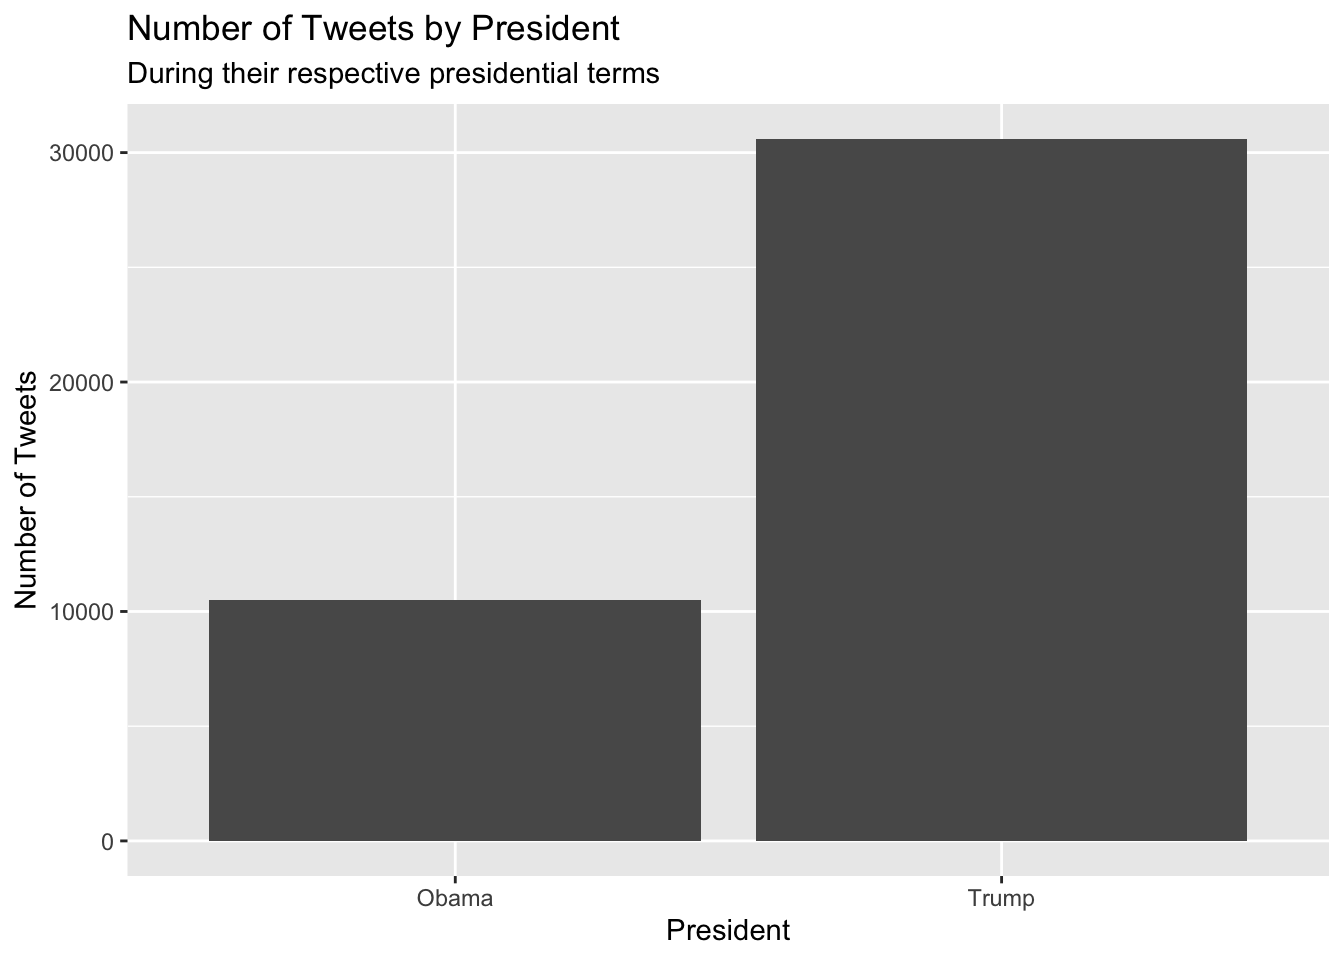
\includegraphics[keepaspectratio]{Mini_Project-3-Strings-and-Sentiment_files/figure-pdf/unnamed-chunk-3-1.pdf}}

These results really surprised me. Even though President Obama served
two terms, he only made 10519 total tweets, while Trump made a whopping
30605 tweets during his one term. It seems like Trump has a big mouth,
and likes to tweet, considering he tweeted three times as much during
his presidency compared to Obama. After seeing how much Obama and Trump
tweeted, let us analyse how frequently they would tweet during their
presidency.

\begin{Shaded}
\begin{Highlighting}[]
\NormalTok{obama\_and\_trump }\SpecialCharTok{|\textgreater{}}
  \FunctionTok{group\_by}\NormalTok{(year\_month, president) }\SpecialCharTok{|\textgreater{}}
  \FunctionTok{count}\NormalTok{() }\SpecialCharTok{|\textgreater{}} 
  \FunctionTok{ggplot}\NormalTok{(}\FunctionTok{aes}\NormalTok{(}\AttributeTok{x =}\NormalTok{ year\_month, }\AttributeTok{y =}\NormalTok{ n)) }\SpecialCharTok{+}
  \FunctionTok{geom\_line}\NormalTok{() }\SpecialCharTok{+}
  \FunctionTok{facet\_wrap}\NormalTok{(}\SpecialCharTok{\textasciitilde{}}\NormalTok{president) }\SpecialCharTok{+}
  \FunctionTok{labs}\NormalTok{(}\AttributeTok{title =} \StringTok{"Frequency of Tweets During Respective Presidency"}\NormalTok{ ,}
         \AttributeTok{x =} \StringTok{"Year"}\NormalTok{, }
       \AttributeTok{y =} \StringTok{"Number of Tweets"}\NormalTok{)}
\end{Highlighting}
\end{Shaded}

\pandocbounded{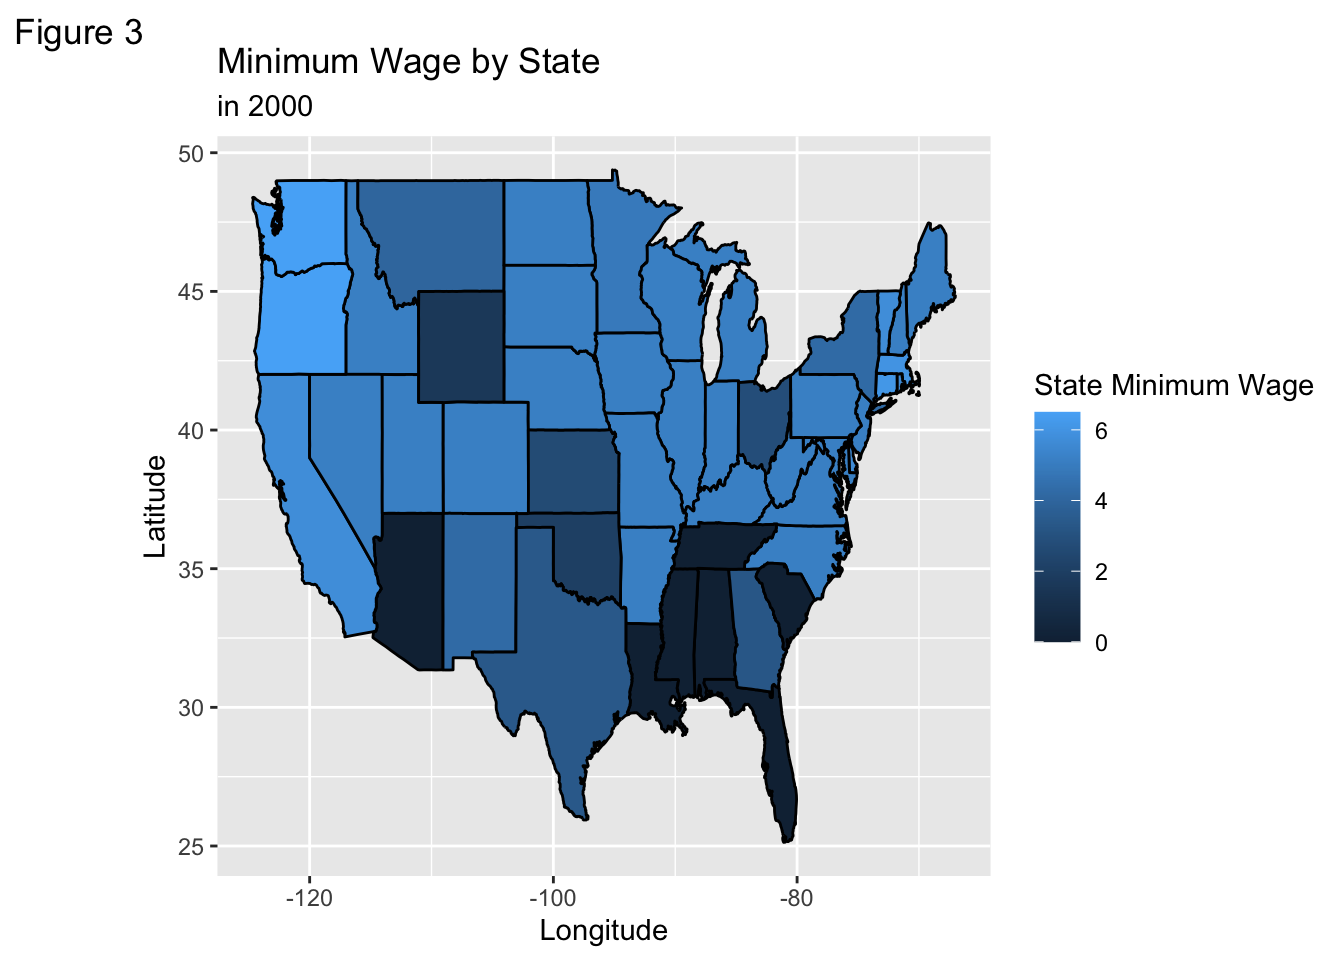
\includegraphics[keepaspectratio]{Mini_Project-3-Strings-and-Sentiment_files/figure-pdf/unnamed-chunk-4-1.pdf}}

Even though Obama and Trump served in different terms, we are still able
to analyse how often each president would tweet. In just the year 2020,
Trump tweeted around 12200 times. Obama did not tweet as much as Trump;
however, this might be because social media was not as widely used
during 2008-2016. His maximum number of tweets was in the year 2012,
with a total of 2652 tweets. As the years went on, social media became
more prevalent to the daily lives of many, which might explain the why
Trump felt the need to tweet more frequently.

After our initial analysis of Obama's and Trump's tweets, we can do more
data wrangling to make the data set more usable. First, let us convert
all the tweets into lower case, and removing the special characters of
``@'', ``\#'', ``:'', quotation marks, etc. In addition to removing
these special characters, I decided to remove any links that are
present. Links offer little to no information, and is not necessary for
our analysis of interest. In order to do more meaningful analysis in
regards to both Obama's and Trump's tweets, let us use the
\texttt{unnest\_tokens} to create a new column of individual words based
on their respective tweets. After creating this new column, we must
remove all the \texttt{stop\_words} or words that provide little to no
importance in sentiment analysis.

\begin{Shaded}
\begin{Highlighting}[]
\NormalTok{obama\_and\_trump }\OtherTok{\textless{}{-}}\NormalTok{ obama\_and\_trump }\SpecialCharTok{|\textgreater{}}
  \FunctionTok{mutate}\NormalTok{(}\AttributeTok{tweet\_lower =} \FunctionTok{str\_to\_lower}\NormalTok{(tweet), }
         \AttributeTok{tweet\_lower =} \FunctionTok{str\_remove\_all}\NormalTok{(tweet\_lower, }\StringTok{"}\SpecialCharTok{\textbackslash{}\textbackslash{}}\StringTok{@"}\NormalTok{),}
         \AttributeTok{tweet\_lower =} \FunctionTok{str\_remove\_all}\NormalTok{(tweet\_lower, }\StringTok{"https.+"}\NormalTok{),}
         \AttributeTok{tweet\_lower =} \FunctionTok{str\_remove\_all}\NormalTok{(tweet\_lower, }\StringTok{"}\SpecialCharTok{\textbackslash{}\textbackslash{}}\StringTok{\#"}\NormalTok{),}
         \AttributeTok{tweet\_lower =} \FunctionTok{str\_remove\_all}\NormalTok{(tweet\_lower, }\StringTok{"}\SpecialCharTok{\textbackslash{}\textbackslash{}}\StringTok{:"}\NormalTok{),}
         \AttributeTok{tweet\_lower =} \FunctionTok{str\_remove\_all}\NormalTok{(tweet\_lower, }\StringTok{\textquotesingle{}"\textquotesingle{}}\NormalTok{)) }\SpecialCharTok{|\textgreater{}} 
  \FunctionTok{filter}\NormalTok{(tweet\_lower }\SpecialCharTok{!=} \StringTok{""}\NormalTok{) }\SpecialCharTok{|\textgreater{}}
  \FunctionTok{unnest\_tokens}\NormalTok{(word, tweet\_lower) }


\NormalTok{obama\_and\_trump }\OtherTok{\textless{}{-}}\NormalTok{ obama\_and\_trump }\SpecialCharTok{|\textgreater{}}
  \FunctionTok{anti\_join}\NormalTok{(stop\_words)}


\NormalTok{word\_list }\OtherTok{\textless{}{-}} \FunctionTok{as\_tibble}\NormalTok{(qdapDictionaries}\SpecialCharTok{::}\NormalTok{DICTIONARY)}


\NormalTok{obama\_and\_trump }\OtherTok{\textless{}{-}}\NormalTok{ obama\_and\_trump }\SpecialCharTok{|\textgreater{}}
  \FunctionTok{semi\_join}\NormalTok{(word\_list) }

\NormalTok{obama\_and\_trump }\OtherTok{\textless{}{-}}\NormalTok{ obama\_and\_trump }\SpecialCharTok{|\textgreater{}}
  \FunctionTok{filter}\NormalTok{(word }\SpecialCharTok{!=} \StringTok{"president"}\NormalTok{, word }\SpecialCharTok{!=} \StringTok{"trump"}\NormalTok{)}
\end{Highlighting}
\end{Shaded}

After removing these special characters and links, I realized that in
some of their tweets, there were either typos, or they were responding
to other Twitter users. Thus, I needed to use the function
\texttt{semi\_join} my \texttt{obama\_and\_trump} data set with
\texttt{DICTIONARY} in the \texttt{qdapDictionaries} library to remove
words that are not are not in the English language. In addition to doing
so, I've decided to remove the words of ``Trump'' and ``president''
because I felt it was unnecessary to include them in my analysis.

\section{Quick Analysis of Names
Mentioned}\label{quick-analysis-of-names-mentioned}

\begin{Shaded}
\begin{Highlighting}[]
\NormalTok{name\_list }\OtherTok{\textless{}{-}} \FunctionTok{as\_tibble}\NormalTok{(qdapDictionaries}\SpecialCharTok{::}\NormalTok{NAMES) }\SpecialCharTok{|\textgreater{}}
  \FunctionTok{rename}\NormalTok{(}\StringTok{"word"} \OtherTok{=} \StringTok{"name"}\NormalTok{) }\SpecialCharTok{|\textgreater{}}
  \FunctionTok{mutate}\NormalTok{(}\AttributeTok{word =} \FunctionTok{str\_to\_lower}\NormalTok{(word))}

\NormalTok{obama\_and\_trump\_names }\OtherTok{\textless{}{-}}\NormalTok{ obama\_and\_trump }\SpecialCharTok{|\textgreater{}}
  \FunctionTok{semi\_join}\NormalTok{(name\_list) }\SpecialCharTok{|\textgreater{}}
  \FunctionTok{rename}\NormalTok{(}\AttributeTok{name =}\NormalTok{ word) }\SpecialCharTok{|\textgreater{}}
  \FunctionTok{filter}\NormalTok{(name }\SpecialCharTok{!=} \StringTok{"america"}\NormalTok{, name }\SpecialCharTok{!=} \StringTok{"china"}\NormalTok{, name }\SpecialCharTok{!=} \StringTok{"florida"}\NormalTok{)}
\end{Highlighting}
\end{Shaded}

\begin{verbatim}
Joining with `by = join_by(word)`
\end{verbatim}

\begin{Shaded}
\begin{Highlighting}[]
\NormalTok{obama\_and\_trump\_names }\SpecialCharTok{|\textgreater{}} 
  \FunctionTok{group\_by}\NormalTok{(president, name) }\SpecialCharTok{|\textgreater{}}
  \FunctionTok{count}\NormalTok{() }\SpecialCharTok{|\textgreater{}}
  \FunctionTok{arrange}\NormalTok{(}\FunctionTok{desc}\NormalTok{(n)) }\SpecialCharTok{|\textgreater{}}
  \FunctionTok{pivot\_wider}\NormalTok{(}\AttributeTok{names\_from =}\NormalTok{ president, }\AttributeTok{values\_from =}\NormalTok{ n ) }
\end{Highlighting}
\end{Shaded}

\begin{verbatim}
# A tibble: 194 x 3
# Groups:   name [194]
   name   Trump Obama
   <chr>  <int> <int>
 1 love     407    77
 2 bill     358   122
 3 mike     214     2
 4 major    206    23
 5 hope     205    27
 6 guy      184     4
 7 chance   124   172
 8 chuck    132     4
 9 mark     122    16
10 page     101    19
# i 184 more rows
\end{verbatim}

Trump talks a lot out Joe and Hillary, while Obama talks a lot about
Michelle.

Since we are doing sentiment analysis, let us implement both the
categorical and numerical emotion scale. We do that with the following
code: \texttt{get\_sentiments("nrc")}, which categorizes words to a
corresponding emotion. \texttt{get\_sentiments("afinn")} categorizes
words numerically, based on how negative or positive the word is.

\texttt{get\_sentiments("nrc")} has ten distinct values: trust, fear,
negative, sadness, anger, surprise, positive, disgust, joy, anticipation
while \texttt{get\_sentiments("afinn")} takes on the value from (-5,5).

\section{Word Cloud for Obama}\label{word-cloud-for-obama}

\begin{Shaded}
\begin{Highlighting}[]
\NormalTok{obama\_and\_trump }\SpecialCharTok{|\textgreater{}} 
  \FunctionTok{filter}\NormalTok{(president }\SpecialCharTok{==} \StringTok{"Obama"}\NormalTok{) }\SpecialCharTok{|\textgreater{}} 
  \FunctionTok{inner\_join}\NormalTok{(}\FunctionTok{get\_sentiments}\NormalTok{(}\StringTok{"bing"}\NormalTok{)) }\SpecialCharTok{|\textgreater{}}
  \FunctionTok{count}\NormalTok{(word, sentiment, }\AttributeTok{sort =} \ConstantTok{TRUE}\NormalTok{) }\SpecialCharTok{|\textgreater{}}
  \FunctionTok{acast}\NormalTok{(word }\SpecialCharTok{\textasciitilde{}}\NormalTok{ sentiment, }\AttributeTok{value.var =} \StringTok{"n"}\NormalTok{, }\AttributeTok{fill =} \DecValTok{0}\NormalTok{) }\SpecialCharTok{|\textgreater{}}
  \FunctionTok{comparison.cloud}\NormalTok{(}\AttributeTok{scale =} \FunctionTok{c}\NormalTok{(}\DecValTok{2}\NormalTok{, .}\DecValTok{5}\NormalTok{), }\AttributeTok{colors =} \FunctionTok{c}\NormalTok{(}\StringTok{"gray80"}\NormalTok{, }\StringTok{"gray20"}\NormalTok{),}
                   \AttributeTok{max.words =} \DecValTok{300}\NormalTok{, }\AttributeTok{title.size =} \DecValTok{1}\NormalTok{)}
\end{Highlighting}
\end{Shaded}

\pandocbounded{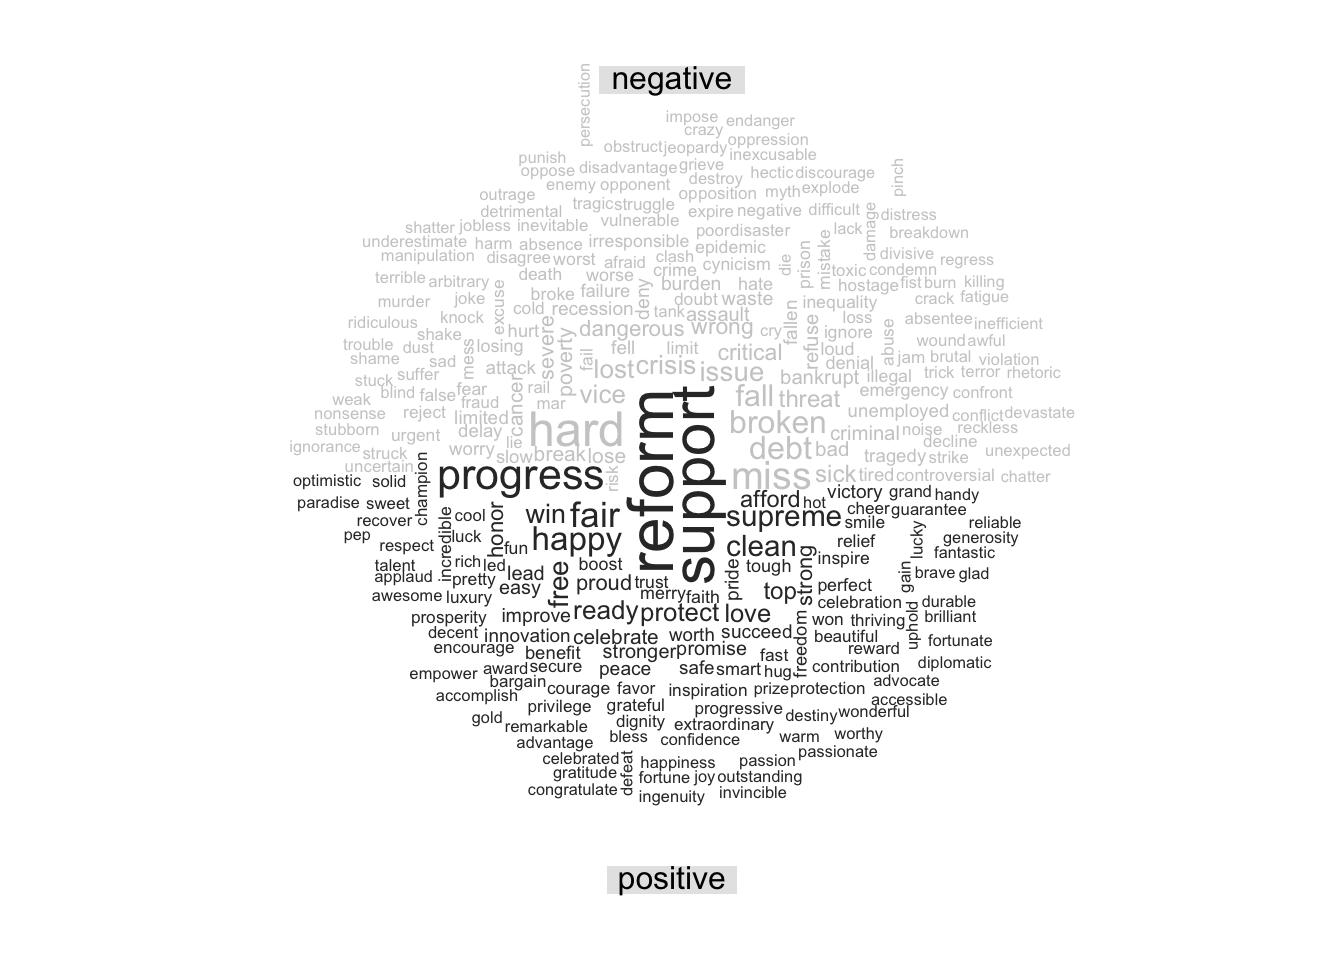
\includegraphics[keepaspectratio]{Mini_Project-3-Strings-and-Sentiment_files/figure-pdf/unnamed-chunk-8-1.pdf}}

Above, we can see the word cloud for Obama; it displays the 300 most
popular words he uses. He uses the words ``support,'' ``reform,'' ''
work,'' ``progress,'' ``protect,'' and ``inspire'' which all have
positive connotations.

\section{Word Cloud for Trump}\label{word-cloud-for-trump}

\begin{Shaded}
\begin{Highlighting}[]
\NormalTok{obama\_and\_trump }\SpecialCharTok{|\textgreater{}} 
  \FunctionTok{filter}\NormalTok{(president }\SpecialCharTok{==} \StringTok{"Trump"}\NormalTok{) }\SpecialCharTok{|\textgreater{}} 
  \FunctionTok{inner\_join}\NormalTok{(}\FunctionTok{get\_sentiments}\NormalTok{(}\StringTok{"bing"}\NormalTok{)) }\SpecialCharTok{|\textgreater{}}
  \FunctionTok{count}\NormalTok{(word, sentiment, }\AttributeTok{sort =} \ConstantTok{TRUE}\NormalTok{) }\SpecialCharTok{|\textgreater{}}
  \FunctionTok{acast}\NormalTok{(word }\SpecialCharTok{\textasciitilde{}}\NormalTok{ sentiment, }\AttributeTok{value.var =} \StringTok{"n"}\NormalTok{, }\AttributeTok{fill =} \DecValTok{0}\NormalTok{) }\SpecialCharTok{|\textgreater{}}
  \FunctionTok{comparison.cloud}\NormalTok{(}\AttributeTok{scale =} \FunctionTok{c}\NormalTok{(}\DecValTok{1}\NormalTok{, .}\DecValTok{5}\NormalTok{), }\AttributeTok{colors =} \FunctionTok{c}\NormalTok{(}\StringTok{"gray80"}\NormalTok{, }\StringTok{"gray20"}\NormalTok{),}
                   \AttributeTok{max.words =} \DecValTok{300}\NormalTok{, }\AttributeTok{title.size =} \DecValTok{1}\NormalTok{)}
\end{Highlighting}
\end{Shaded}

\pandocbounded{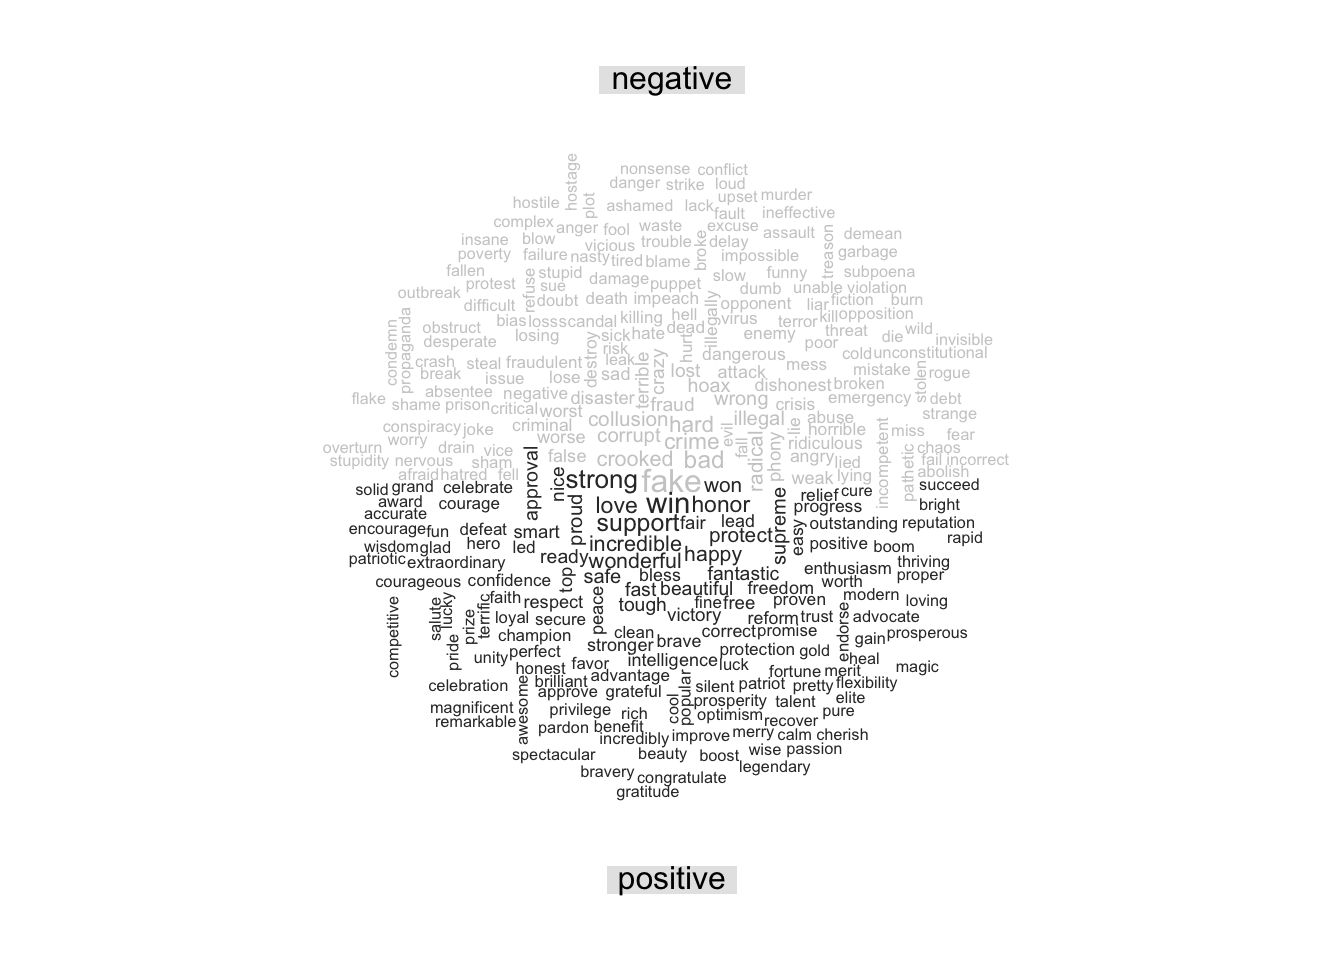
\includegraphics[keepaspectratio]{Mini_Project-3-Strings-and-Sentiment_files/figure-pdf/unnamed-chunk-9-1.pdf}}

Trump's word cloud shows that some of this popular words are also
``support,'' ``great,'' ``stronger,'' ``protection,'' ``honor,'' and
``wonderful''.

When comparing the word clouds of the two, I was surprised about how
hard it is to make out some of the words in Trumps cloud. His most
popular word seems to be the word ``great,'' however, I think it is
attributed to his slogan. From the word cloud alone, one can easily tell
that Obama talked about ``support,'' ``reform,'' ``progress,'' ``work,''
``debt,'' and ``broken'' most of the time because these words are the
biggest. In Trump's case however, it is harder to tell what he would
tweet about, since there are no clear standouts.

\section{Sentiment Analysis}\label{sentiment-analysis}

How do presidents talk on Twitter? On average, how often do they use
words with negative connotations, and how often do they use words with
positive connotations? Is there a difference between the two. We begin
our analysis by joining our data set with the ``nrc'' sentiments tibble.

\begin{Shaded}
\begin{Highlighting}[]
\NormalTok{pres\_analysis }\OtherTok{\textless{}{-}}\NormalTok{ obama\_and\_trump }\SpecialCharTok{|\textgreater{}} 
  \FunctionTok{inner\_join}\NormalTok{(}\FunctionTok{get\_sentiments}\NormalTok{(}\StringTok{"nrc"}\NormalTok{), }\AttributeTok{relationship =} \StringTok{"many{-}to{-}many"}\NormalTok{)}

\NormalTok{n1 }\OtherTok{\textless{}{-}}\NormalTok{ pres\_analysis }\SpecialCharTok{|\textgreater{}}
  \FunctionTok{filter}\NormalTok{(president }\SpecialCharTok{==} \StringTok{"Obama"}\NormalTok{) }\SpecialCharTok{|\textgreater{}}
  \FunctionTok{count}\NormalTok{(sentiment) }\SpecialCharTok{|\textgreater{}} 
  \FunctionTok{mutate}\NormalTok{(}\AttributeTok{sentiment =} \FunctionTok{fct\_reorder}\NormalTok{(sentiment, n)) }\SpecialCharTok{|\textgreater{}} 
  \FunctionTok{ggplot}\NormalTok{(}\FunctionTok{aes}\NormalTok{(}\AttributeTok{x =}\NormalTok{ sentiment, }\AttributeTok{y =}\NormalTok{ n, }\AttributeTok{fill =}\NormalTok{ sentiment)) }\SpecialCharTok{+}
  \FunctionTok{geom\_col}\NormalTok{(}\AttributeTok{show.legend =}  \ConstantTok{FALSE}\NormalTok{) }\SpecialCharTok{+} 
  \FunctionTok{theme}\NormalTok{(}\AttributeTok{axis.text.x =} \FunctionTok{element\_text}\NormalTok{(}\AttributeTok{angle =} \DecValTok{60}\NormalTok{, }\AttributeTok{hjust =} \FloatTok{0.5}\NormalTok{, }\AttributeTok{vjust =} \FloatTok{0.5}\NormalTok{)) }\SpecialCharTok{+} 
  \FunctionTok{ylim}\NormalTok{(}\DecValTok{0}\NormalTok{, }\DecValTok{30000}\NormalTok{) }\SpecialCharTok{+} 
  \FunctionTok{labs}\NormalTok{(}\AttributeTok{x=}\StringTok{"Sentiment"}\NormalTok{, }\AttributeTok{y=}\StringTok{"Count"}\NormalTok{, }\AttributeTok{title=} \StringTok{"Obama"}\NormalTok{)}


\NormalTok{n2 }\OtherTok{\textless{}{-}}\NormalTok{ pres\_analysis }\SpecialCharTok{|\textgreater{}}
  \FunctionTok{filter}\NormalTok{(president }\SpecialCharTok{==} \StringTok{"Trump"}\NormalTok{) }\SpecialCharTok{|\textgreater{}}
  \FunctionTok{count}\NormalTok{(sentiment) }\SpecialCharTok{|\textgreater{}}
  \FunctionTok{mutate}\NormalTok{(}\AttributeTok{sentiment =} \FunctionTok{fct\_reorder}\NormalTok{(sentiment, n)) }\SpecialCharTok{|\textgreater{}} 
  \FunctionTok{ggplot}\NormalTok{(}\FunctionTok{aes}\NormalTok{(}\AttributeTok{x =}\NormalTok{ sentiment, }\AttributeTok{y =}\NormalTok{ n, }\AttributeTok{fill=}\NormalTok{sentiment)) }\SpecialCharTok{+}
  \FunctionTok{geom\_col}\NormalTok{(}\AttributeTok{show.legend =} \ConstantTok{FALSE}\NormalTok{) }\SpecialCharTok{+} 
  \FunctionTok{theme}\NormalTok{(}\AttributeTok{axis.text.x =} \FunctionTok{element\_text}\NormalTok{(}\AttributeTok{angle =} \DecValTok{60}\NormalTok{, }\AttributeTok{hjust =} \FloatTok{0.5}\NormalTok{, }\AttributeTok{vjust =} \FloatTok{0.5}\NormalTok{)) }\SpecialCharTok{+} 
  \FunctionTok{labs}\NormalTok{(}\AttributeTok{x =} \StringTok{"Sentiment"}\NormalTok{, }\AttributeTok{y =} \StringTok{"Count"}\NormalTok{, }\AttributeTok{title=} \StringTok{"Trump"}\NormalTok{)}

\FunctionTok{grid.arrange}\NormalTok{(n1, n2, }\AttributeTok{nrow=}\DecValTok{1}\NormalTok{)}
\end{Highlighting}
\end{Shaded}

\pandocbounded{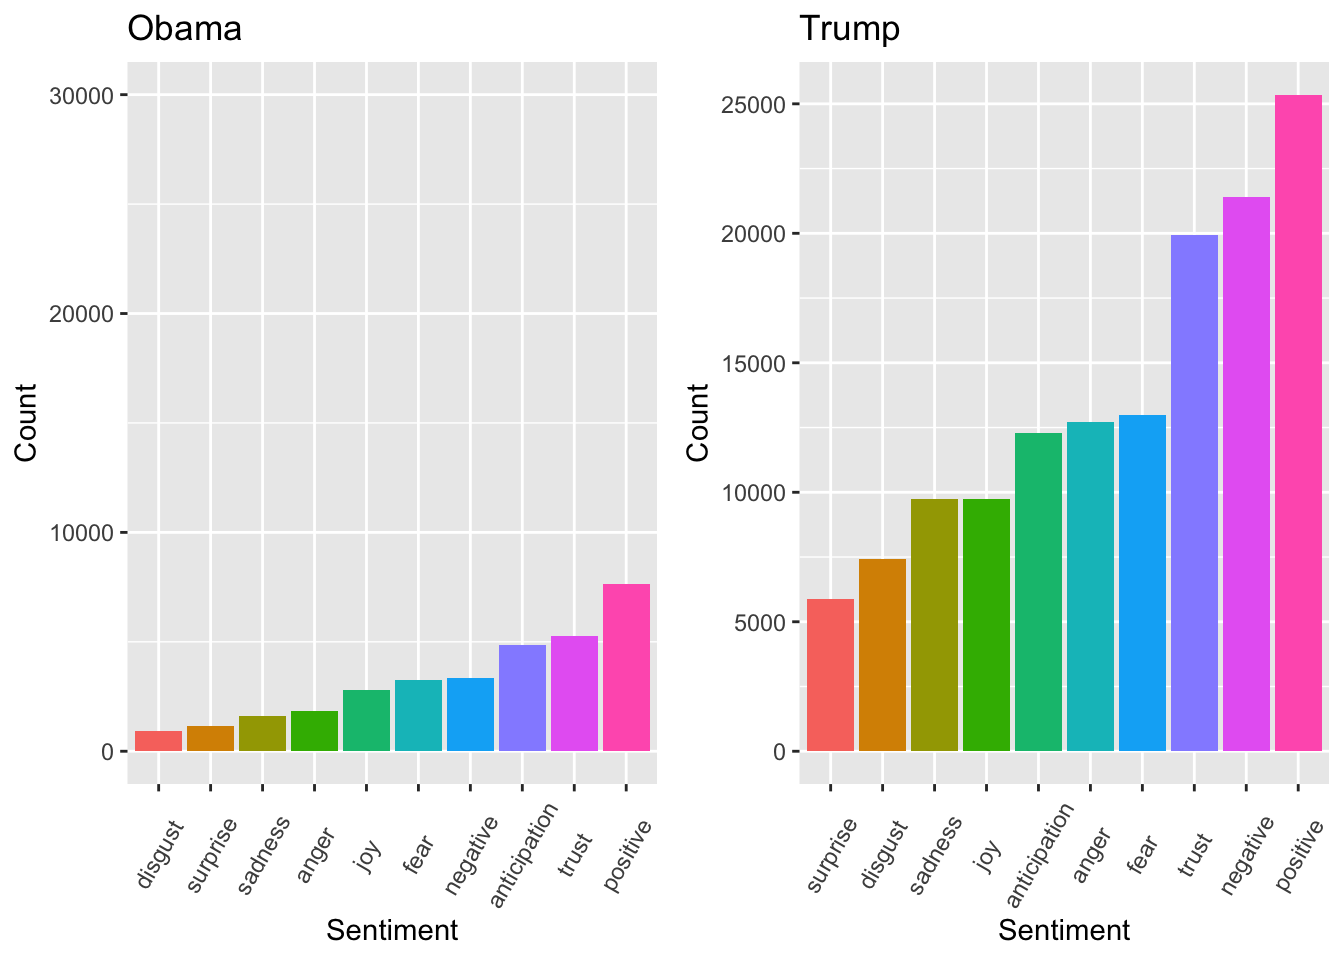
\includegraphics[keepaspectratio]{Mini_Project-3-Strings-and-Sentiment_files/figure-pdf/unnamed-chunk-10-1.pdf}}

The figure above shows how often each president would use words with a
certain sentiment. It seems Obama regularly words that are associated
with positivity, trust, anticipation and negativity. While Trump
regularly used words that are associated with positivity, negativity,
trust, anticipation and fear.\\
It is surprising to see that Trump used a comparable number of words
with positive and negative connotations. An important factor to consider
is that the data is influenced by Trump's greater volume of tweets
compared to Obama's. While it may appear that Trump exhibited more
positive tweeting behavior, this observation may not be entirely
accurate.

In addition to exploring their respective sentiment, I was curious on
how their would change with respect to time.

\begin{Shaded}
\begin{Highlighting}[]
\NormalTok{pres\_year\_analysis }\OtherTok{\textless{}{-}}\NormalTok{ obama\_and\_trump }\SpecialCharTok{|\textgreater{}} 
  \FunctionTok{inner\_join}\NormalTok{(}\FunctionTok{get\_sentiments}\NormalTok{(}\StringTok{"bing"}\NormalTok{), }\AttributeTok{relationship =} \StringTok{"many{-}to{-}many"}\NormalTok{)}

\NormalTok{t1 }\OtherTok{\textless{}{-}}\NormalTok{ pres\_year\_analysis }\SpecialCharTok{|\textgreater{}} 
  \FunctionTok{filter}\NormalTok{(president }\SpecialCharTok{==} \StringTok{"Obama"}\NormalTok{) }\SpecialCharTok{|\textgreater{}} 
  \FunctionTok{group\_by}\NormalTok{(year\_month) }\SpecialCharTok{|\textgreater{}} 
  \FunctionTok{count}\NormalTok{(sentiment) }\SpecialCharTok{|\textgreater{}}
  \FunctionTok{spread}\NormalTok{(sentiment, n) }\SpecialCharTok{|\textgreater{}}
  \FunctionTok{mutate}\NormalTok{(}\AttributeTok{score =}\NormalTok{ positive }\SpecialCharTok{{-}}\NormalTok{ negative) }\SpecialCharTok{|\textgreater{}}
  \FunctionTok{drop\_na}\NormalTok{() }\SpecialCharTok{|\textgreater{}} 
  \FunctionTok{ggplot}\NormalTok{(}\FunctionTok{aes}\NormalTok{(}\AttributeTok{x =}\NormalTok{ year\_month, }\AttributeTok{y =}\NormalTok{ score)) }\SpecialCharTok{+}
  \FunctionTok{scale\_x\_date}\NormalTok{(}\AttributeTok{limits=}\FunctionTok{c}\NormalTok{(}\FunctionTok{as.Date}\NormalTok{(}\StringTok{"2008{-}03{-}01"}\NormalTok{), }\FunctionTok{as.Date}\NormalTok{(}\StringTok{"2016{-}12{-}31"}\NormalTok{)), }\AttributeTok{date\_breaks =} \StringTok{"3 month"}\NormalTok{, }\AttributeTok{date\_labels =} \StringTok{"\%b"}\NormalTok{) }\SpecialCharTok{+} 
  \FunctionTok{geom\_line}\NormalTok{(}\AttributeTok{stat=}\StringTok{"identity"}\NormalTok{, }\AttributeTok{col=}\StringTok{"blue"}\NormalTok{) }\SpecialCharTok{+} \FunctionTok{geom\_smooth}\NormalTok{(}\AttributeTok{col=}\StringTok{"red"}\NormalTok{) }\SpecialCharTok{+} 
  \FunctionTok{labs}\NormalTok{(}\AttributeTok{title=}\StringTok{"Sentiment Barack Obama"}\NormalTok{) }\SpecialCharTok{+} 
  \FunctionTok{theme}\NormalTok{(}\AttributeTok{axis.text.x =} \FunctionTok{element\_text}\NormalTok{(}\AttributeTok{angle =} \DecValTok{45}\NormalTok{, }\AttributeTok{hjust =} \DecValTok{1}\NormalTok{))}

\NormalTok{t2 }\OtherTok{\textless{}{-}}\NormalTok{ pres\_year\_analysis }\SpecialCharTok{|\textgreater{}} 
  \FunctionTok{filter}\NormalTok{(president }\SpecialCharTok{==} \StringTok{"Trump"}\NormalTok{) }\SpecialCharTok{|\textgreater{}} 
  \FunctionTok{group\_by}\NormalTok{(year\_month) }\SpecialCharTok{|\textgreater{}} 
  \FunctionTok{count}\NormalTok{(sentiment) }\SpecialCharTok{|\textgreater{}}
  \FunctionTok{spread}\NormalTok{(sentiment, n) }\SpecialCharTok{|\textgreater{}}
  \FunctionTok{mutate}\NormalTok{(}\AttributeTok{score =}\NormalTok{ positive }\SpecialCharTok{{-}}\NormalTok{ negative) }\SpecialCharTok{|\textgreater{}}
  \FunctionTok{drop\_na}\NormalTok{() }\SpecialCharTok{|\textgreater{}} 
  \FunctionTok{ggplot}\NormalTok{(}\FunctionTok{aes}\NormalTok{(}\AttributeTok{x =}\NormalTok{ year\_month, }\AttributeTok{y =}\NormalTok{ score)) }\SpecialCharTok{+}
  \FunctionTok{scale\_x\_date}\NormalTok{(}\AttributeTok{limits=}\FunctionTok{c}\NormalTok{(}\FunctionTok{as.Date}\NormalTok{(}\StringTok{"2016{-}01{-}01"}\NormalTok{), }\FunctionTok{as.Date}\NormalTok{(}\StringTok{"2021{-}01{-}01"}\NormalTok{)), }\AttributeTok{date\_breaks =} \StringTok{"3 month"}\NormalTok{, }\AttributeTok{date\_labels =} \StringTok{"\%b"}\NormalTok{) }\SpecialCharTok{+} 
  \FunctionTok{geom\_line}\NormalTok{(}\AttributeTok{stat=}\StringTok{"identity"}\NormalTok{, }\AttributeTok{col=}\StringTok{"blue"}\NormalTok{) }\SpecialCharTok{+} \FunctionTok{geom\_smooth}\NormalTok{(}\AttributeTok{col=}\StringTok{"red"}\NormalTok{) }\SpecialCharTok{+} 
  \FunctionTok{labs}\NormalTok{(}\AttributeTok{title =}\StringTok{"Sentiment Donald Trump"}\NormalTok{) }\SpecialCharTok{+} 
  \FunctionTok{theme}\NormalTok{(}\AttributeTok{axis.text.x =} \FunctionTok{element\_text}\NormalTok{(}\AttributeTok{angle =} \DecValTok{45}\NormalTok{, }\AttributeTok{hjust =} \DecValTok{1}\NormalTok{))}



\FunctionTok{grid.arrange}\NormalTok{(t1, t2, }\AttributeTok{ncol=}\DecValTok{1}\NormalTok{)}
\end{Highlighting}
\end{Shaded}

\pandocbounded{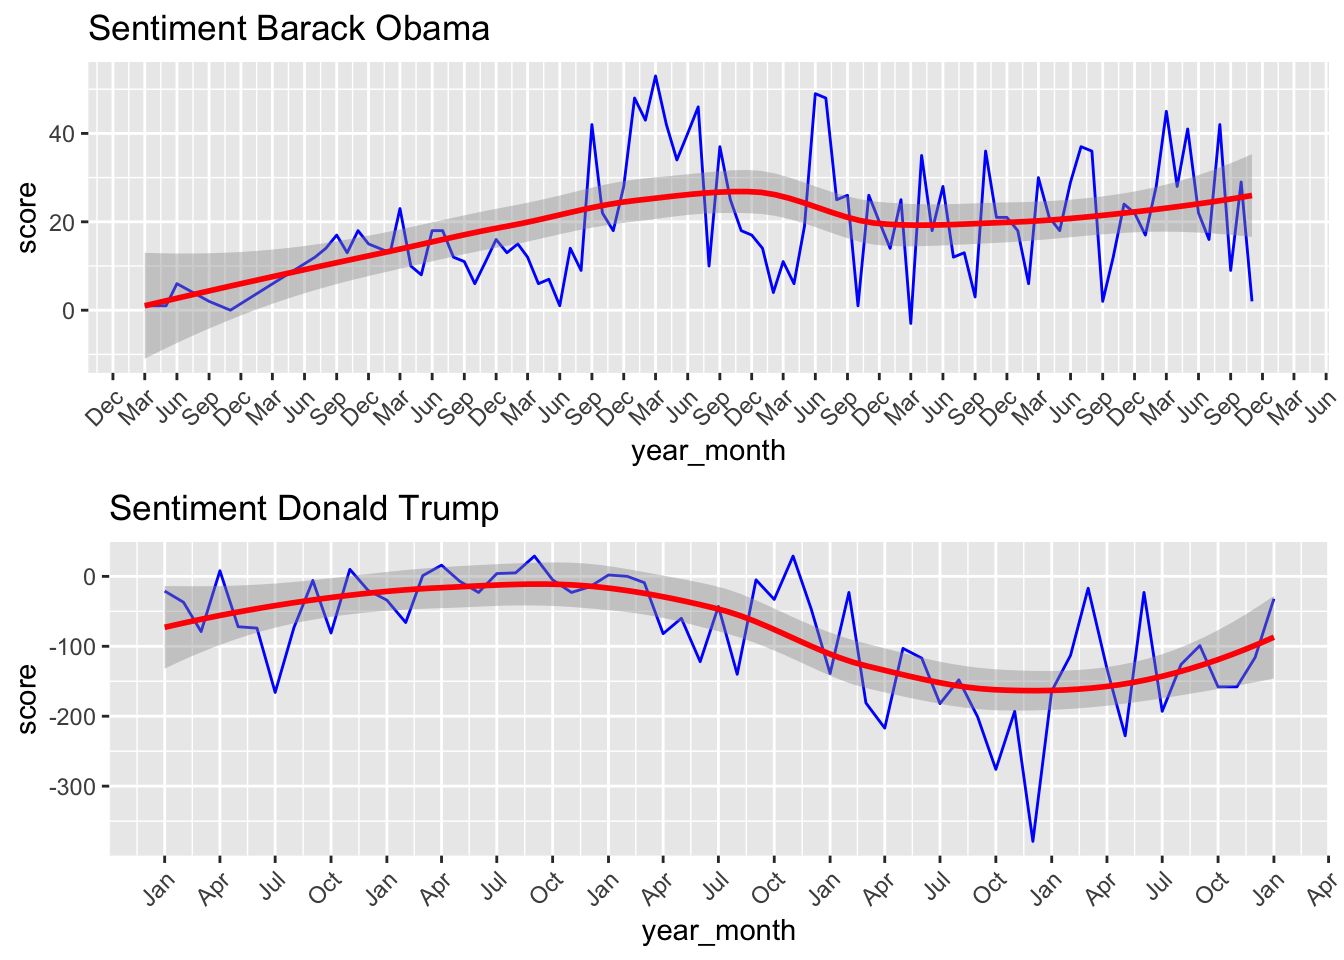
\includegraphics[keepaspectratio]{Mini_Project-3-Strings-and-Sentiment_files/figure-pdf/unnamed-chunk-11-1.pdf}}

The figure above illustrates how Obama's and Trump's sentiment changed
throughout their respective term. Notice how Obama's graph has way more
points on the x-axis, this is because he served two terms, as opposed to
one term. Obama's uses more positive words; the graph shows there is a
slight upward trend in his sentiment score.

However, in the case of Trump, his sentiment score was more variable,
which is also shown in the light gray band, which shows the standard
error of the points. Trump's standard error is bigger, which indicates
that we expect that our estimate of his sentiment score is more variable
than that of Obama's. Around April of 2019, Trump had a sentiment score
of around 350; however, just by doing a quick Google search regarding
his tweets, they are far from positive.

Again, similar to the last graph, notice how it seems like Trump's
sentiment score is higher than Obama's; however, this is due to Trump's
massive amount of tweets.

\section{Conclusion}\label{conclusion}

Although it was fun and interesting to perform sentiment analysis on
both President Obama and President Trump, we have to remember that all
of these words are taken out of context. Even though it seems like one
president has a higher sentiment score, it might not be a reality. If I
were to do a similar kind of sentiment analysis in the future, I would
definitely include phrases such as their campaign slogans. It would have
been more interesting to see if there were certain phrases that they
would say, or even mention a particular country a significant amount.
Also it is important to notice that the results of the analysis is very
skewed because Trump tweeted far more than Obama, which might make it
appear like one person had a higher sentiment score than the other.

\subsection{References:}\label{references}

\begin{itemize}
\tightlist
\item
  \href{https://www.kaggle.com/datasets/neelgajare/all-12000-president-obama-tweets}{Obama
  Tweets:}
\item
  \href{https://www.kaggle.com/datasets/zusmani/trumps-legacy}{Trump
  Tweets:}
\end{itemize}




\end{document}
